% 来源：OEBPS/Text/Section0001_split_005.xhtml#sigil_toc_id_38

\BookChapter{26}
\section[第26章\q 打不垮，沉不了，压不住：全天候投资策略]{第26章\\ 打不垮，沉不了，压不住：全天候投资策略}

\begin{BookQuote}
不可胜者，守也。

\hfill ——《孙子兵法》
\end{BookQuote}

我们人生中有些事件，永远地塑造了我们的世界观。这就像我们旅途中公路上的公里标志，不管我们是否能看懂它的意思，它都给了我们一个视角来看现在的世界。我们选择的那些事件对于我们而言具有什么样的意义，将会像涟漪一样影响到我们的行为和决定，这种影响会持续我们一生。

如果你是在咆哮的20世纪20年代长大的，这十年里巨大的繁荣和伟大的事件会塑造你的人生。那是伟大的“盖茨比”的年代。但是如果你是在接下来大萧条的20世纪30年代长大的，那么那个时代充斥的挣扎和焦虑会把你的人生塑造成另外一个样子。成长在一个严酷的经济寒冬，逼迫你变成一个求生者。

现在这个时代的人对整个世界有着完全不同的体验。他们成长在不可思议的繁荣之中，即使他们的收入并不属于前1/100的富豪，他们也活得非常幸福。我们生活在一个需求方说了算的世界，作为消费者能够享受到巨大的便利。我们可以让日用杂货商品直接快递到我们家门口，舒舒服服地穿着睡衣就能将收到的支票存到自己的银行账户，看的电视有上千个频道，什么时间、什么地方的节目你都能看，只要你想看。我的孙女到现在还没有学会系鞋带，但是她刚4岁的时候就能把iPad（苹果平板电脑）玩得跟我这个爷爷一样好，她已经知道，谷歌只用一小会儿就能够回答任何问题。这是一个无限可能的时代，一个创业企业，例如网络信使只有50多名员工，但它可以颠覆一个行业，因此这个企业的收购价格高达190亿美元。

毫无疑问，我们生活的时代的发展情况和重大事件塑造了我们的人生，但是更重要的是，我们赋予这些事件的意义将会决定我们最终的发展轨迹。

\subsection{20世纪70年代}

瑞·达利欧1949年出生，2014年时已经65岁。他在20世纪70年代开始做投资。20世纪70年代经济发展形势出现巨大变化，可以说是20世纪30年代大萧条以来最糟糕的经济环境。高失业率伴随着巨大的通货膨胀，导致利率水平像火箭一样飙升，竟然高达百分之十几。你还记得，我在高通货膨胀的20世纪70年代买了房，借的抵押贷款的利率是18\%，高得吓人！1973年美国又迎来一场石油危机，美国根本没有料到，阿拉伯国家会对美国实行石油禁运，导致油价从每桶2.1美元飙升到10.4美元。没有一个人预料到会发生这样的事情。美国政府强制进行汽油单双号配给制，迫使人们不仅排队加油要等上好几个小时，而且只能在单号或者双号的日子去加油！这是一个政治上激烈斗争的时期，经历了越南战争和水门事件之后，美国人民对政府的信任大幅度降低。1974年尼克松总统被迫辞职，后来他的继任者，也就是前任副总统杰拉德·福特特赦了他。

1971年，瑞·达利欧刚从大学毕业，第一份工作是进入纽约证券交易所当一名小职员。身在市场中，他亲眼看到牛市和熊市在短时间内爆发，创造出巨大的市场波动性，让各种不同的资产类型都大幅波动。潮水突如其来，又匆匆而去，人们根本无法预测。达利欧看到了巨大的收益机会，但是他也看到了同样巨大甚至更加巨大的风险，巨大的风险与机会并存在这片巨大的海域里。结果，他变得极其痴迷于想要弄明白，所有这些场景和波动是如何交织在一起的。在理解更大的经济机器是如何运转的过程中，他最终弄明白了如何避免那些像遭到大洪水一样的巨大损失，这让很多投资者注定失败。

所有这些事件塑造了年轻的瑞·达利欧，让他最终成为世界上规模最大的对冲基金经理。但是，有个对塑造达利欧的投资哲学影响最大的顿悟时刻，它出现在1971年8月一个酷热的晚上，尼克松总统突然发表演讲，从而改变了我们习以为常的金融世界。

\subsection{尼克松之夜}

美国三大广播电视网，突然中断正在播出的所有节目，美国总统尼克松突然出现在所有美国家庭客厅的电视机屏幕上和收音机里。很明显，他处于一种严肃又焦虑的状态，他宣布：“我命令国务卿约翰·康纳利暂时停止美元兑换黄金。”只有简短的一句话，20多个字，美国总统尼克松向全世界宣布，我们熟悉的美元再也不会是以前的样子了，美元的价值再也不和黄金直接挂钩了。还记得诺克斯堡吗？这个城堡的作用就是，对于政府印发的每一张美元纸钞，美国政府都会持有相同价值的实物黄金，这些黄金就保存在这个城堡内，它被严密保护。但是当尼克松这样宣布美元和黄金脱钩时，美元从那时开始就只是一张纸了。想象一下，本来你有个藏宝箱，里面装满了黄金，结果有一天你打开一看，发现一张一张黄色的便利贴，上面只写着两个字：欠条。

尼克松说，现在决定美元价值的是我们，即市场。市场认为美元价值多少，美元就值多少。这个新闻也震惊了其他国家的政府，它们持有大量美元，一直相信可以随时选择把美元兑换成黄金。一夜之间，尼克松公开地把这种选择权拿掉了，这倒是非常符合他的外号“狡猾的迪克”。他还宣布对所有进口的商品额外征收10\%的关税，以保证美国国内产品的市场竞争力。就像10月末的一场暴风雪，尼克松的演讲标志着气候的巨大变化。

瑞·达利欧正在家里看电视，看到美国总统的演讲，他简直不敢相信他的耳朵所听到的。尼克松决定让美国脱离金本位，这会产生什么影响？这对市场意味着什么？对美元和美元在全世界的地位意味着什么？

有一点，瑞·达利欧敢肯定：“这意味着钱的定义不同了，我想也许会有一场危机！”他内心想，第二天早上他一走进交易所，肯定会看到，整个市场暴跌。

他错了。

让他震惊的是，道琼斯指数第二天涨了接近4\%，股票指数涨幅创下了有史以来最大单日涨幅，黄金价格也像火箭一样飙升！这完全是违背直觉的，大多数专家的预测都错了。毕竟我们刚刚毁掉的是我们对全世界的神圣承诺，这些上面印有已故美国总统头像的纸片，实际上是有实际价值的。当然，这种变化不会激发人们对美国经济和美国政府的信心。这是一件让人头疼的事情，这次市场繁荣最终名扬天下，被称为“尼克松大反弹”。

但这带来的并不都是好消息。“我们认为美元价值是多少，它就价值多少。”这导致一场通货膨胀风暴正在酝酿，不久就会到来。达利欧详细地描述道：“但是当时是在1973年，第一次石油禁运危机就种下了严重通货膨胀的祸根。我们以前从来没有担心过石油危机。我们以前从来没有担心过通货膨胀。所有这些事情，在感觉上都成了意外。我发展形成了一套预测意外的方法。”另外，这是指那种我们承受不了的意外，或者说我们没有能力化解的意外。就像下一个2008年金融危机。这种意外就是下一个冲击波，它肯定会让我们整个市场大动荡。

尼克松反弹成了瑞·达利欧的人生催化剂：他从此开始执着于对任何事情做好准备，包括全世界任何一个角落，随处都可能会发生的你根本不知道的事情。他的使命是，研究任何一种可以想象得到的市场环境，这对某些投资来说意味着什么。这是他的核心操作原则，他靠这个原则来管理世界上最大的对冲基金。不是依靠他已经知道的东西，而是正好相反。他总是不满足地、充满饥渴地持续寻找他所不知道的东西。因为明显的东西往往是明显错误的。普遍流行的思想常常是错误的思想。因为世界是持续改变和进化的，瑞·达利欧探索未知的旅程是一条永远没有终点的探索之路。

\subsection{终极投资极乐世界}

你接下来要读到的内容，很可能会是整本书中最重要的一章。是的，我知道，我以前也这样说过好多次了。我每次说都是真的。如果你不知道游戏的规则，你就会让对手击倒，把你撕得粉碎。如果你不是像一个内行一样思考，传统的智慧会引导你接受类似大众的命运。如果你没有决定把一部分收入的一定比例拿出来，让你的储蓄自动化，你的火箭就永远飞不起来，其中的原因很简单——燃料不够。但是我发自内心地完全相信本书里讲的内容，没有什么能够比得上瑞·达利欧设计的这个投资策略，让你可能获得的收益最大化，却同时让你承受的风险最小化。这正是瑞·达利欧的特别之处。这也正是达利欧名扬世界的秘密所在。

你在下面学到的投资组合，能给你提供以下三大好处：

第一，非凡的高收益性——最近40年（1974—2013年）里年化收益率接近10\%，（精确地说是扣费后9.88\%）。

第二，非凡的高安全性——最近40年85\%的时间里，你的资金都是安全的，只有6个年度出现了亏损，平均亏损幅度只有1.47\%。6次亏损中有两个年度，其实是盈亏平衡，因为有一年亏了0.03\%，还有一年亏得更少，无论怎么看，它都属于盈亏平衡。所以从实践操作的角度来看，这40年你其实只有4年是亏钱的。

第三，非凡的低波动性——最近40年你能体验的最糟糕的亏损，也只有3.93\%。

还记得沃伦·巴菲特的投资终极法则吗？第一条，不要亏钱；第二条，牢记第一条。实际运用巴菲特这个投资法则的，正是瑞·达利欧的天赋所在，这正是为什么他能成为投资界的达·芬奇。

任何人都能向你展示一个投资组合，（事后来看）你要承担巨大的风险，才能得到高收益，如果组合下跌50\%\textasciitilde{}60\%的时候，你的勇气没有像个纸袋一样瘪下去，而是一直坚定地持有，你最终肯定会有很大的投资收益。这个建议，基金和券商在做市场营销时说起来非常好听，但是对于大多数人来说很难做到，一点儿也不现实。

我简直不能想象，竟然有这样一种方法，适合你我这样的个人投资者，让我们能够获得像股票市场整体水平一样的收益率。与此同时，还有一种策略能够最大限度地限制损失的发生频率和规模，几乎能让你安然度过每一种可以想象到的经济环境。你能想象到，竟然有一种投资组合模式，在2008年只亏损了3.93\%吗？要知道2008年当时整个世界都崩溃了，股票市场从顶点暴跌50\%。有一个投资组合，你这样投资之后，会感到非常安全和安稳，即使再发生下一个2008年金融危机这个让人吓得魂飞魄散的大崩盘，席卷走美国人退休金账户上数万亿股票市值，你也能安然无忧。这就是我要送给你的礼物，它就在后面的内容里。（过去的业绩并不能保证未来的业绩，相反，我提供给你的是历史数据，用来讨论和描述投资的基本原则。）

我们很快就会揭开这个神奇的投资组合，让你欣赏到瑞·达利欧投资之道的美妙和力量，在此之前，让我们先了解一下瑞·达利欧这个人的故事，他可是我们所在的地球上神奇得简直不可思议的投资和资产配置的绝顶高手。全世界各国政府和世界上最大的公司，电话快速拨号键上都存着瑞·达利欧的电话，以便它们能够及时咨询如何把它们的收益最大化，同时使它们的损失最小化。

\subsection{我就爱麦乐鸡}

1973年，对于小鸡来说，真是个倒霉的年头。正是在那一年，麦当劳决定推出麦乐鸡，结果产品卖疯了。这让麦当劳花了好几年才能解决供应链的问题，没办法，因为公司无法获得那么多鸡肉。但如果不是瑞·达利欧给出天才般的解决方案，麦乐鸡根本无法继续卖。

光鲜亮丽的投资界怎么会跟快餐业掺和在一起？这是因为麦当劳要推出麦乐鸡这款新品，管理层非常焦虑，害怕以后鸡肉的成本上升，这样就会提高鸡肉的价格。但是那些经常光顾麦当劳的顾客，花钱都是很节省的，麦当劳想让套餐提价，这些顾客可不干，马上就会离开。但是鸡肉供应商不愿意接受固定价格，因为他们知道，不是鸡的价格高了，关键是喂养小鸡用的那些玉米和大豆的饲料成本的价格提高了。如果饲料成本上涨，卖给麦当劳的鸡肉价格固定不变，供应商就必须自己消化这些损失。

麦当劳的人给瑞·达利欧打电话求助，因为他们知道达利欧是世界上最有才的家伙，他最大的天才就是让你的上行潜在收益最大化，与此同时，消除风险或者把风险最小化。瑞·达利欧在电话里给出了一个解决办法。他设计出一份私人定制的期货交易合约（简单说就是一个保证，避免未来玉米和大豆价格上涨），这样就能让鸡肉供应商得到固定价格的玉米和大豆供应，于是那些供应商就乐于和麦当劳签订合同，按照固定价格供应鸡肉。大家共同获利。祝你好胃口！

瑞·达利欧专业能力的影响范围远远超出麦当劳这样的大公司。你想知道他的智慧在全世界的影响有多么深远吗？1997年，美国财政部决定发行能够抵抗通货膨胀的债券（现在它们一般被称为TIPS）。美国财政部官员专门来到瑞·达利欧的公司——桥水基金公司，向他咨询如何来设计这些债券产品。瑞·达利欧的建议构成了现在通用的保值债券基本条款的结构。

瑞·达利欧不只是一个基金管理人，他在市场研究和风险管理上也是大师，他知道如何选择不同的交易价格，以便获胜的概率极其有利于自己和客户。

达利欧是怎么做到的？他的秘密是什么？让我们坐下来，靠近这位投资大师，让他带我们踏上这趟投资智慧之旅吧。

\subsection{智慧海豹突击队}

还记得吗，我在开篇讲过，瑞·达利欧给了我们一个丛林的比喻？就像达利欧看到的那样，如果我们想要到达我们真正想去的地方，我们必须穿越丛林。丛林是危险的，因为里面有很多东西我们都一无所知，有些挑战就隐藏在下个转弯的地方，它们会伤害到你。但是为了到达你真正想要去的地方，你必须在你周围聚集一些你很尊敬的、世界顶级聪明的头脑。瑞·达利欧创办的桥水基金公司，就是他个人组建的“丛林高手”团队。他的桥水基金公司员工超过1500名，个个都和达利欧一样，非常痴迷于如何找到办法，既让收益最大化，又把风险最小化。

前面我说过，桥水基金公司是世界上规模最大的对冲基金公司，管理规模超过1600亿美元。这个规模在业内是极大的了，现在管理规模能超过150亿美元都算得上大型对冲基金了，桥水基金公司一家的规模就超过10家大型对冲基金公司。尽管一般投资者根本没有听说过瑞·达利欧，但是他的名字在顶级财富圈里十分响亮。瑞·达利欧写的投资评论、简报，就是金融圈最有权势的大人物也会阅读，其中包括各国中央银行的行长，也包括各国政府的高官，甚至是美国总统。

因此，全世界最大规模的机构，包括规模最大的养老基金、外国主权财富基金，都把很多资金交给达利欧来管理和投资。大家都想了解达利欧的投资高见。为什么？关键是瑞·达利欧想的、说的、做的，并不是传统智慧的所思所想。他能跳出既有观念来思考，甚至会粉碎那些条条框框。他总是非常饥渴地持续学习和挑战传统的东西，发现“真理”是推动达利欧持续快速增长的动力，让他从最早的只拥有公寓兼办公室，一路成长到拥有康乃狄格一片蜿蜒的巨大校区。他在桥水基金公司组建的丛林团队被称为智慧海豹突击队。在桥水工作，你要和瑞·达利欧一起穿越丛林，并肩战斗。桥水基金公司的文化要求你要有创造性、洞察力和勇气——总是能够捍卫你的投资立场和投资观点。但是达利欧也要求你，必须主动质疑，甚至攻击任何你觉得错误的事情。你的使命就是找出什么是真相，然后找出最好的办法来处理和应对真相。这种工作方式要求“彻底开放，彻底真实，彻底透明”。整个公司的生存和成功都得益于此。

\subsection{阿尔法狗}

瑞·达利欧之所以名扬天下，靠的是他的纯阿尔法策略对冲基金取得的非凡成功。1991年他推出这个对冲基金，现在管理规模达到800亿美元，年化收益率21\%（扣费前），高得令人难以置信，风险却相对较低。基金的投资者包括世界上最富有的个人、政府、养老基金。这些投资人的资产规模可以说是1\%中的1\%的1\%。这个“小圈子”已经停止接收新投资人很多年了。纯阿尔法策略对冲基金是主动管理型的，这意味着达利欧和他的团队在持续不断地寻找投资机会，他们想在正确的时间进入，在正确的时间退出。桥水基金并不只是跟随市场，有一点可以作为例证，那就是2008年他们获得了17\%的收益率（扣费前），而很多对冲基金管理公司都关门了，或者乞求投资者不要赎回，不然公司就会破产。纯阿尔法策略基金的投资者，希望得到更大的收益，也愿意为这些投资承担风险——尽管他们还是尽自己最大努力地在最大限度地控制他们承担的风险。

\subsection{孩子和慈善}

瑞·达利欧管理纯阿尔法策略对冲基金，取得了不可思议的成功，帮客户赚了很多钱，这也让他赚了很多钱，积累了巨大的个人财富。1995年前后，他开始考虑自己可以给后代留下什么遗产，留下什么样的基金，但是他心里疑惑的是：“如果我人不在了，不能坐在这里主动管理这些资金，那么我该运用什么类型的投资组合？”什么样的投资组合，可以比他自己做投资决策能活得更久，而且继续创造良好的收益，以继续支撑他的孩子成长，以及慈善事业所需要的花费？

达利欧知道，传统智慧和传统的投资组合管理，会把他的方法构建成一个投资模型，而历史数据持续表明，碰到市场变得异常糟糕的时候，这个投资模型就不适用了。所以他开始探索是否可以创建一个组合（就是一种资产配置）在将来的任何经济情况下都能做得很好，不管是像2008年那样严酷的经济寒冬还是经济衰退，甚至是经济萧条。没有人知道再过5年会发生什么，更不用说再过20年、30年了。

结果是什么？

换一种全新的方式来看资产配置，设计出一套全新的规则。达利欧先是用长期历史市场行情来测试这个策略，一直回测到1925年，结果令他很满意。然后达利欧再将这个策略用在个人管理的家庭信托投资上，结果产生了辉煌的业绩，经受了多种经济情况的考验。经过双重考验之后，他才用这个策略推出了一只对冲基金，只限于少数经过选择的投资人。其中的条件之一是这些人每人至少要投资1亿美元。这个新的策略，名为全天候投资策略，1996年才第一次公开亮相，仅仅过了4年，网络股泡沫破裂，股市三年暴跌一半，这个新的策略面临严峻考验。结果全天候投资策略顺利地通过考验，业绩表现非常出色。

\subsection{问题就是答案}

我们都听过那句格言：“问，你就会得到答案。”但是如果你问的是更好的问题，你得到的答案也会更好，这是所有取得重大成功人士的共同特点。比尔·盖茨问的问题不是“怎么样才能打造世界上最棒的软件”，他问的是“我怎么样才能创造出一套操作系统控制所有的计算机”。这两个问题的区别就决定了微软不但成为最成功的软件公司，还成了主导计算机世界的力量——目前仍然控制着全球90\%的个人计算机市场！不过比尔·盖茨没有掌握网络，因为他把专注点放在了计算机上面。但是创办谷歌搜索的两个男孩拉里·佩奇和索杰·布林问的是：“我们如何组织安排全世界的信息，让信息随手可得、随时可用？”结果他们专注于一个更加强大的力量，这个力量深度影响了科技、生活、商业。你问的问题层次越高，更高层次的回报才会随之而来。要得到结果，你不能只问一次，你必须变得非常执迷于给这个问题寻找伟大的答案（很多个答案）。

一般人问的问题都是这样的：“这件事我怎样才能应付过去？”“为什么这件事情会发生在我身上？”有些人甚至问的问题是负能量的，他们的头脑关注和发现的是障碍，而不是寻找解决方案。这种负能量的问题是：“我怎么从来都减不掉体重？”“为什么我从来都管不住自己花钱？”这样只能让他们在自我限制的路上走得更远。

我一直非常执着于这个问题：我如何能把事情做得更好？我如何帮助人们现在就能明显地改善他们的生活品质？这个关注点驱动我过去38年来寻找和创建策略和工具，不是以后见效，而是马上见效。你呢？哪个（哪些）问题你问的比别的问题加在一起还要多？你最关注的是什么？你人生中最痴迷的是什么，寻找真爱，与众不同，学习，赚钱，让每个人都高兴，避免痛苦，改变世界？你意识到你最关注的问题是什么了？你认识到你一生最重要的问题是什么了吗？不管你一生最关注的是什么，都会塑造、框定、指导你的人生。本书回答的问题是：“那些最高效的投资人做了什么能让他们持续获得成功？”这些人原来也一无所有，但是想方设法地创造出巨大的财富和财务自由，让他们的家人能够分享，那么他们在这个过程中做出的决策和采取的行动是什么？

在金融世界里，瑞·达利欧变得非常痴迷于一系列更高质量的问题。这些问题导致他最终创造出了全天候投资组合。这正是你很快就会在本书中学到的投资方法，这个投资方法法力无边，有能力从此改变你的财务人生，从此你的财务人生会变得更好。

“设计一个什么样的投资组合，让人可以绝对地确定，不管经济状况是好还是坏，都能表现良好——穿越所有的经济环境？”

这也许听起来是个显而易见的问题，事实上很多所谓的“专家”和财务顾问都会说，他们正在使用分散的资产配置，设计的目的就是要做到这一点。但是，正是用传统的答案来回答这个问题，导致很多专业投资机构会在2008年亏损30\%\textasciitilde{}50\%，我们看到很多目标日期基金遭到大屠杀，而按照设计，它们本来应该是，持有人越接近设定的退休年纪，其持有的基金投资组合应该越保守，结果是应该保守却远远不够保守。我们也看到，雷曼兄弟，这个有158年历史的基石型金融机构，几天就垮掉了。在那个时候，大多数投资理财顾问躲到桌子底下，不敢接听客户打来的电话。我的一个朋友开了个苦涩的玩笑：“我的401(k)退休金账户现在跌成了一个201（k）。”金融行业使用的所有梦幻般的软件——用蒙特卡洛模拟计算所有类型的潜在未来情景，那些巨大的危机既没有被预测到，也没有被防卫，结果让投资者亏惨了，例如1987年股市黑色星期一大崩盘，2000年网络股泡沫大崩盘，2008年金融危机毁灭性大崩盘，名单还很长。

你要是重新回忆一下2008年那些日子，你听到的标准回答都是这样的：“这种事以前从来没有发生过。”“我们现在是在从来没有人探索过的海域。”“这次和以前完全不一样。”瑞·达利欧根本不理睬这些回答（这也正是为什么他预测到了2008年全球性金融危机，还在2008年赚到了大钱）。

不要误解瑞·达利欧所说的“意外”——这一次总是看起来跟上一次不一样。1973年石油禁运危机，20世纪70年代后期快速通货膨胀，1976年英镑危机，1987年黑色星期一，2000年网络股泡沫，2008年房地产崩盘，所有这些意外，都让大多数专业人士猝不及防。下一次意外还会来临，还会让他们摔个大跟头。这一点我们完全可以肯定。

但是2009年当烟雾散去后，市场开始反弹，很少有资金管理人停止追问，他们原来使用的传统资产配置方式和风险管理是不是从一开始就是错的。有很多人拍拍身上的灰尘，重新骑上销售的马鞍，口里又开始念念有词，一切将回到“常态”。但是请记住瑞·达利欧的投资魔咒“预料意外”，还有他的核心操作问题“什么是我不知道的”。问题不是将来会不会再有一次大崩盘，问题是大崩盘什么时候会来。

\subsection{马科维茨：收益最大化的秘密}

哈里·马科维茨，人称现代投资组合理论之父，这套理论让他获得诺贝尔经济学奖。他这样解释现代投资组合理论背后的基本概念。简单来说，你要是看你投资组合里的投资，不能只是单个来看，而应该从整体来看。这里面有一个风险和收益之间的权衡，所以就像听交响乐一样不能只听一种乐器的声音，你要听整个乐团合在一起演奏出的声音。你的那些投资个体的不同表现，加上投资分散的情况，二者最终决定你的组合的总体收益情况。这个建议现在听起来也许太简单了，但是在1952年这种想法简直是“新大陆”。在某种程度上，这个道理影响了从纽约到香港全世界每一个投资组合的经理人。

和所有伟大的投资人一样，瑞·达利欧站在了马科维茨的肩膀上，用他的核心智慧作为基础，来考虑任何投资组合或者资产配置的设计。但是他还想把它再提升到更高的水平上。他可以肯定，他肯定能够增加一两个关键的特质——拉动两个关键的杠杆，创造出属于他自己的突破性发现。他用自己40年的投资经验，召集桥水基金公司的丛林战队，把他们的脑力投注在这个开发计划上。达利欧可以说是花了很多年来不断地精进他的研究，直到最终找到了一种全新的方式来看待资产配置。这就是终极资产配置，完美的资产配置，既收益最大化又风险最小化。瑞·达利欧的发现，给他自己创造出一种全新水平的竞争优势——你很快也会拥有这种竞争优势。

瑞·达利欧这种改变人生也改变游戏的投资方法，一直秘不外传，只有他的客户才能享受到这种独门绝招带来的好处。政府、养老金管理机构、亿万富豪，作为达利欧的客户，都从这个策略中享受到了非凡的投资收益，全靠这一招。不用再羡慕，你很快也能学到瑞·达利欧的全天候投资策略。就像我前面所说过的，这就是瑞·达利欧在金钱游戏中用的神奇盔甲。达利欧把他的家庭和慈善基金的所有资金，都投进这种投资组合，再加上世界上最保守、最资深的金融机构委托他管理的安全/安心水桶里面的资金，就像瑞·达利欧那样，我现在也把我家庭的一部分资金用这种方式进行投资，包括我的基金会的资金，原因很简单，它非常赚钱。你会开始看到，在近85年的各种经济环境下，这个策略都产生了良好的业绩。从经济萧条到经济衰退，再到通货膨胀和通货紧缩，无论经济形势的好坏，这个策略都能找到一种方法，找到投资机会把投资收益最大化。从历史数据来看，这是最好的投资方式之一，它可能会实现我的愿望，即使是在我离世很久之后它也能正常运作。

\subsection{游戏日}

瑞·达利欧可以称得上我们这个时代伟大的投资传奇人物之一，能有机会当面向他请教，确实是一份难得的馈赠，我可得好好利用。我花了将近15个小时做研究，充分准备我跟瑞·达利欧的见面，梳理我手上能够找到的各种资料（这事很不好办，因为他一直回避媒体，不愿公开露面）。我挖掘出来一些瑞·达利欧少有的几次演讲：一次是在达沃斯论坛上对世界各国领导人发表的演讲，一次是对美国国会对外关系委员会发表的演讲。我也看了查理·罗斯在《60分钟》节目中对他的访谈，这是他仅有的几次媒体亮相之一。我也看了他指导的动画视频《经济机器是如何运作的：30分钟全掌握》。这是一段很棒的视频节目，我强烈建议你看一看，有助于你真正理解整个世界经济是怎么运作的。我能找到他写的每一篇白皮书和文章，我全看了，还仔细梳理了一篇。他写过一本小书，其实是一篇长文，书名是《原则》，内容包括他的人生和投资管理指导原则，我仔细阅读，差不多每一页都在上面做了标记，画了重点。这是一生只有一次的机会，我不能让自己未完全做好准备，就去见这位最伟大的投资大师。

原来说好是一个小时的采访，很快变成接近三个小时。我一点儿也没想到，达利欧竟然还是我的粉丝，喜欢我写的书，一直在听我的音频教程，听了近20年了。我简直太荣幸了！我们越谈越深。你来我往，你说我答，我们谈的内容也越来越广，从投资扩大到世界经济这台大机器实际上是如何运行的。我一开始问了一个简单的问题：“对于个人投资者来说，这个游戏还能赢吗？”

“能！”瑞·达利欧说，加重语气，肯定地说。但是你肯定不能听你认识的那个经纪人小帅哥给你的建议，照着他说的做，那你肯定赢不了投资游戏。你若想靠预测市场涨跌来选择进入市场的时机，这样你肯定也赢不了这个投资游戏。你若想预测市场，基本上就是跟全世界最优秀的选手来玩扑克牌，他们拥有几乎无穷无尽的资源，可以跟你玩上几天几夜，无论是能力、经验、资源、时间，你都差远了，想赢是不可能的。在牌桌上就只有这么多玩扑克牌的筹码，“这是一个零和游戏”。有人赢多少，肯定就有人输多少。所以，你想要从像达利欧这样的投资高手的手里赢走一些筹码，那简直是痴心妄想，你只是一厢情愿而已。“这是一个全世界的人都在参与的大赛，但只有极少数人能够实实在在地赚到钱，他们赚了很多钱，不过都是从那些没有他们优秀的选手手里赚走的。”正如人们常说的，如果你在一张牌桌上玩了一会儿，还没有看出来谁是傻瓜，那么你就是那个傻瓜。

很多人想要努力战胜市场，想要预测市场，瑞·达利欧给这些人一个终极警告：“你根本不应该参加那种游戏。”

“好了，达利欧，我们知道了我们这些业余投资者不应该妄想战胜世界上最好的投资职业高手，那么我要问你一个问题，我为写本书访谈过的专业人士，我都问过这个问题，如果你不能留给你的孩子任何钱，而只能给他们一个投资组合清单，一个具体的资产配置清单，加上一个投资原则清单来指导他们投资，你给他们的清单会是什么？

达利欧往后坐了坐，我可以看出他迟疑了一会儿，并不是他不想分享，而是因为我们生活在一个无比复杂的世界中，这里充满机会，也充满风险。“托尼，只是这事太复杂了。事情在不断变化，在这样的情况下，只用很短的时间把这个问题给普通的投资人讲明白，对于我来说非常难。”

“是的，达利欧，我理解你的难处。但是你也刚刚告诉过我，个人投资者要是买基金，找一个传统的基金经理是不可能取得成功的。所以请你讲讲，帮我们弄明白，我们能做些什么才能取得成功。我们都知道资产配置是我们投资成功的最重要因素，那么你用的是哪些基本原则让你创造的收益最大化，同时又让风险最小化呢？”

正是在这个时候，瑞·达利欧开始敞开心扉，分享一些惊人的投资秘密和投资高见。他的第一步是粉碎我的传统智慧，向我证明了传统智慧认为的平衡投资组合，其实并不平衡。

\begin{BookQuote}
所有胜利的秘密都隐藏在隐秘之中。

\hfill ——马可·奥勒留
\end{BookQuote}

\subsection{不平衡}

大多数投资顾问（还有广告）会鼓励你去拥有一个“平衡的”投资组合。平衡，听起来像是一件好事，对吧？平衡告诉我们，我们不会承受太多的风险。那我们较大风险的投资，会让我们较保守的投资把风险对冲掉。但是问题来了：市场暴跌的时候，为什么最传统的平衡投资组合竟然会下跌25\%\textasciitilde{}40\%，并没有平衡巨大的下跌风险？

传统的平衡投资组合，一般是这样配置的：50\%的股票和50\%的债券（如果以更加激进一些的话可以是60∶40；或者如果你更加激进的话，可以是70∶30）。让我们就一直用50∶50为例，这样举例更好理解。这意味着如果有个人手上有1万美元，她会把5000美元投在股票上，5000美元投在债券上。同样，如果他有10万美元的话，那就是5万美元投到债券上，5万美元投到股票上。你应该明白了，反正就是一半股票对一半债券。

用这种典型的平衡方式，我们希望做到以下三点：

第一，我们希望股票表现良好。

第二，我们希望债券表现良好。

第三，我们希望下一波市场崩溃来临时，不要股票债券两个同时下跌——股债双杀。

你很容易注意到，希望是这种传统投资之道的基础，但是投资内行，像瑞·达利欧，并不依赖于希望。希望不是策略，不能靠希望来为你的家庭赚取投资收益。

\subsection{买股票投资企业有风险}

把你的资金分配成50\%的股票对50\%的债券（或者其他的总体配置比例），很多人认为他们已经分散投资了，分散开了他们的风险。但是事实的真相是，你真的承受了太多的风险，比你想的多得多。为什么？因为就像瑞·达利欧在我们谈话中多次强调指出的那样，股票风险要比债券风险高3倍（这里说的风险就是波动性）。

“托尼，持有一半股票一半债券的组合，你其实是让这一半股票承担整个组合95\%的风险！”下面是两个饼图，代表的50∶50的投资组合的资金配置和风险配置。左边这个饼图显示的是资金分别配置到股票和债券上的百分比，右边这张图显示的是同一投资组合股票和债券分别承担的风险比例。

\begin{figure}[htbp]
\centering
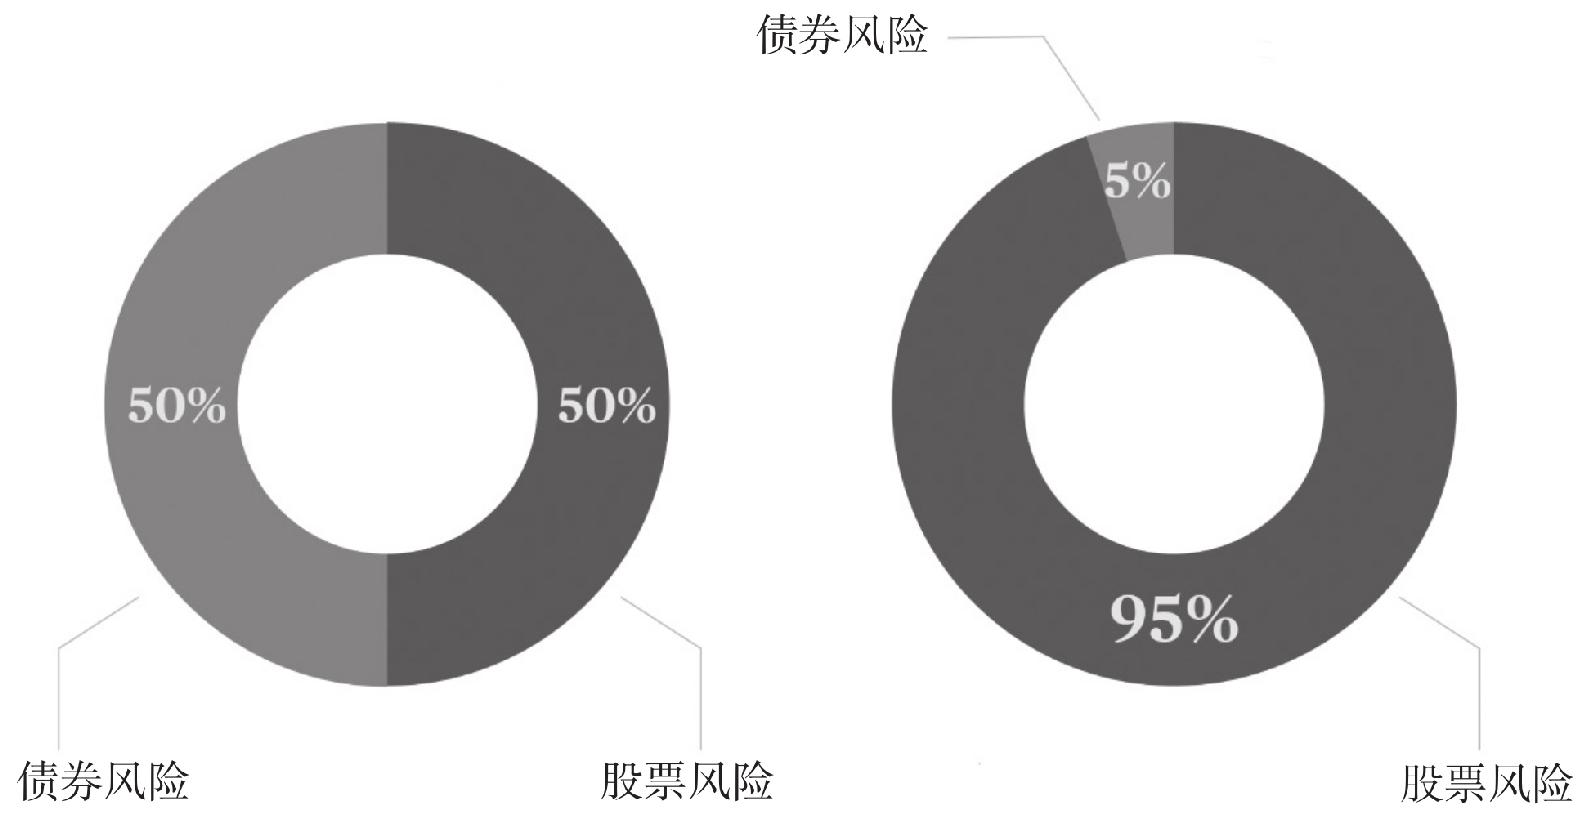
\includegraphics[width=0.76\linewidth,keepaspectratio]{image/26-1.jpg}
\caption{}\label{fig:26-1}
\end{figure}

所以，你把自己资产的50\%配置在股票上，另外50\%配置在债券上，第一眼看好像已经相对平衡了。但是正如右边风险配置那张图显示的那样，你其实承担了接近95\%甚至更大的风险，因为你持有的股票规模和波动性都很大。这样配置，如果股市下跌的话，整个投资组合也会下跌。这其实只是看起来平衡了风险，其实风险还很大。

这个概念怎么体现在现实生活中？

1973—2013年，共有40个年度，其中标准普尔500指数有9个年度都是下跌的，累计跌幅达134\%！同期债券（用伯克利债券指数来代表）只有三年是下跌的，累计亏损只有6\%，所以如果你持有一个50\%股票对50\%债券的投资组合，那么从整体亏损来看，代表股票的标准普尔500指数给你带来的亏损要占到95\%。

“托尼，”瑞·达利欧说，“你自己看看大多数投资组合，它们都有一个非常强烈的偏斜趋势，在股市场行情好的时候组合表现得很好，在股市行情糟糕的时候组合表现得非常糟糕。”所以你的实际策略就是希望股市能上涨。用这种传统的投资方式来做分散投资，其实并没有做到真正分散风险。

我从来没有听过有人能把这种平衡和风险的概念解释得这么简单明了。我坐在那里开始思考我自己的投资：我做了哪些错误的假设？

那么我想问问你，听瑞·达利欧这样解释真正的风险和平衡，你肯定能听明白。那么你觉得自己原来认为“平衡的”投资组合还平衡吗？

这是不是改变了你对平衡的看法？这也意味着改变了你对如何才能真正分散投资风险的看法。我真的希望如此！大多数人会努力保护自己，做法是把资金分散投资到某些不同类型的资产上，分别投入相同数量的资金。有人可能会说：“我的钱50\%放在有风险的股票上（如果经济发展良好的话，股票可能会有更大的上行潜力），50\%的钱放在安全的债券上来保护我。”瑞·达利欧证明给我们看，你的钱分成相同的两部分，但是你的投资风险并没有因此就分成了相同的两半，所以并没有实现平衡！你还是把你大部分的钱置于风险之中，你分配资金的时候必须要根据其风险收益比的高低，而不仅是每个资产类型，投资相同的金额。

你现在知道了一些99\%的投资人甚至是大多数专业投资人都不知道，更没有这样做的内容。但是你不必感觉糟糕。瑞·达利欧说，大多数机构，尽管管理规模高达千亿美元，现在也犯着和你相同的错误！

\subsection{跳舞求雨的原始人}

瑞·达利欧现在进入了状态，越讲越放得开。他开始系统地剖析很多传统的投资误区，这些年来别人一直在向我教授或者说兜售这些东西！

“托尼，平衡投资组合‘理论’还有一个大问题。这套理论的基础建立在一个巨大的、不幸的、错误的假设上。这就是相关性和因果性之间的差别。”

相关性是一个很“高大上”的投资词语，用来描述几种东西一起移动。在原始文化中，原始人会跳舞向老天爷求雨。有的时候它真的显灵了！我们一跳舞，老天爷马上就下雨！或者他们心里是这样想的。其实他们混淆了因果性和相关性。换句话说，他们觉得是他们跳舞这个原因导致老天下雨这个结果，但是其实这只是时间上的巧合而已。如果这种事情一次又一次地发生，次数多了，他们就会形成一些错误的信念，觉得自己有能力预测他们跳舞和下雨之间的相关性。

投资专家也经常陷入同样的迷信误区。他们说有些投资要么是相关的，要么就是不相关的。相关的就会有关联地一起变动，不相关的就是没有可以预测的关联性。是的，有的时候他们也许是相关的，但是就像跳舞求雨的原始人一样，这经常只是巧合而已。

达利欧和他的团队已经证明，历史数据指出的事实是很多投资完全是随机相关的。原来投资界普遍有个假设，股票和债券是负相关的，经常会向反方向发展。2008年的金融危机一下子摧毁了这种非常明显的假设，那一年几乎所有资产类型都完全一致地向下暴跌。真相是有的时候不同类型的资产，比如股票和债券会反向移动，有的时候它们不是这样的，会向同一方向移动。所以当投资专家试图创造平衡，比如他们希望股票走势与债券走势正好完全相反，并且一定会这样，这完全靠运气。但是这种有错误的逻辑推论，却成了大多数金融投资专家投资操作的基本原则。

瑞·达利欧清楚地揭示出，传统的资产配置模型存在一些明显的漏洞。如果他是一个常春藤商学院的教授，把这些东西写成书出版，他可能因此会获得诺贝尔经济学奖提名！但是战士要在战壕里——要待在丛林里——瑞·达利欧更愿意待在这样的地方。

\subsection{投资四季}

我和戴维·斯文森这位耶鲁大学的首席投资官交流的时候，他告诉我：“非传统智慧是唯一一条能让你成功的路。”追随大众，你就根本没有机会成功。人们经常听到同样的建议，想了一遍又一遍，次数多了，就错把这些东西当成了真相，但是正是非传统智慧经常引领我们找到真相，经常引领我们获得一种竞争优势。

这个时候，瑞·达利欧讲出了他的第二个非传统投资智慧：“你回头看看历史，有件事我们绝对可以肯定：每一只投资股都会遇到一种理想的环境。遇到这种环境，这种投资就爆发了。换句话说，每样东西都有自己的好季节。”

比如房地产。21世纪刚开始那几年，美国人简直是见到什么房子就会买什么房子（哪怕是那些根本没有钱的人也会见了房子就买）。他们买房子并不仅是因为利率很低，2009年利率更低，却没有人买房子，他们手上的房子怎么卖也卖不掉。人们在经济繁荣的时候狂买房子是因为房价在快速上涨。房价每个月都在上涨，他们不想错过这样的发大财的机会。百亿富豪、投资大腕儿乔治·索罗斯指出：“美国人2001—2007年这6年里增加的房地产抵押贷款债务总额，比抵押贷款市场创立以来历史累积形成的债务总额还要多。”这是真的，这6年所发放的买房贷款，比此前买房贷款问世以来100多年里发放的所有房贷加在一起还要多。

在迈阿密还有南佛罗里达州的很多地区，你只要付一笔买房的定金，后来因为房价暴涨，还没等到房子建造好，你就可以把没有建好的房子卖掉，获得相当大的利润。人们原来抵押贷款买的房子的市场价格涨了，贷款越还越少，房子的市场价值扣掉贷款价值形成的房产净值越来越大，人们会拿这种房产净值怎么办？他们会二次抵押，贷款去消费、买车、给孩子交学费，其实就把房子当作自动取款机，不断从中变现，然后把钱花掉。由此出现一波巨大的消费增长，由此刺激提升公司的盈利能力，从而进一步推动整个美国经济的增长。索罗斯引用了一些令人吃惊的数字：“美国国会经济顾问委员会的前任主席马丁·菲尔德斯坦估计，1997—2006年消费者把自己的房子做二次抵押贷款，从他们的房屋净值里面变现资金总额超过9万亿美元。”为了让你看明白这一点，我们来用数字说话：只用了6年时间（2001—2007年）美国人房屋抵押贷款增加约5.5万亿美元，超过此前抵押贷款市场100多年整个历史上发生的抵押贷款总额，简单来说，美国房产抵押贷款实现了飞跃，6年超过此前的100年。当然，这种全国性的举动并不是可持续的发展方式。后来房价像块石头一样坠落，消费和经济也随之快速坠落。

总之，哪个季节或者哪种环境会强有力地推动房屋价格上涨？答案是通货膨胀。但是在2009年我们遇到了通货紧缩，结果房价大跌。很多人不再还抵押贷款，把房子扔给银行，因为房价落到水面以下了——现在房子的价格还不够还他们欠银行的贷款。正是通货紧缩让这类房产投资的价格大跌。

股票怎么样？股票在通货膨胀期间也表现良好。通货膨胀来了就会推动物价上涨，更高的物价意味着生产商品和服务的上市公司有机会赚到更多的利润。而公司更高的利润意味着股价上涨。长期以来，事实都证明确实是这样一环套一环的，通货膨胀推动股市一波接一波地上涨。

债券则完全不同，它更喜欢通货紧缩，例如美国国债。如果我们碰到通货紧缩的季节，经常伴随利率下降，债券价格就会上涨。

达利欧揭示了所有这些资产类型最简单也是最重要的区别。只有四种情况能够推动资产的价格变化。

1.通货膨胀

2.通货紧缩

3.提高经济增长率

4.降低经济增长率

% 来源：OEBPS/Text/Section0001_split_005.xhtml → image_ded5a3df005c4711add2735fa137f2d0.jpg
\begin{BookFigureTable}
\begin{longtable}{@{}C{\dimexpr 0.16000\linewidth-1.33333\tabcolsep\relax}C{\dimexpr 0.42000\linewidth-1.33333\tabcolsep\relax}C{\dimexpr 0.42000\linewidth-1.33333\tabcolsep\relax}@{}}
\caption{}\label{fig:26-2}\\
\toprule\noalign{\vskip 3pt}
{\heiti } & {\heiti 增长} & {\heiti 通货膨胀} \\
\midrule
\endfirsthead
\multicolumn{3}{r}{续表}\\[0.6em]
\toprule\noalign{\vskip 3pt}
{\heiti } & {\heiti 增长} & {\heiti 通货膨胀} \\
\midrule
\endhead
\bottomrule
\endfoot
\bottomrule
\endlastfoot
上升 ↑ & 经济增长高于预期 & 通货膨胀高于预期 \\
\midrule
下降 ↓ & 经济增长低于预期 & 通货膨胀低于预期 \\
\end{longtable}
\end{BookFigureTable}


瑞·达利欧的观点归结为4种经济季节，代表可能出现的4种不同的经济环境，它们最终会影响投资（资产价格）上涨或者下跌。“不过有一点不像大自然的四季，这里并没有一个预先设定好的顺序，让你一看就知道接下来哪个季节会到来。”

1.通货膨胀高于预期（价格上涨）

2.通货膨胀（或者通货紧缩）低于预期

3.经济增长率高于预期

4.经济增长率低于预期

你看一看股票或者债券的价格，现在的价格已经包含我们（即市场）对未来的“预期”。达利欧对我说：“托尼，这里有一个关于未来的大致看法，你可以从现在的价格中看到。”换句话说，今天，苹果公司股票的价格已经包含了投资者的预期，他们相信公司会继续按照某个速度增长，因此，你会看到，如果一家公司未来（盈利）增长低于公司原来的预期，就会导致股价大跌，跌幅会大大超过公司预期盈利的跌幅。

“‘意外’最终决定了哪个资产类型会表现良好。如果我们有一个相当好的高增长，这种意外对于股票来说就是惊喜。这对于股票来说简直太好了，但是这对债券就不是那么好了。对于债券来说，如果我们有一个通货膨胀率下降的意外，那就是好事，就是惊喜。”

达利欧说，如果只有这样4种潜在的经济季节或者说是4种经济环境，那么你应该把你的风险分成4个等份，分别配置到4个季节各自最有利的不同类型的资产上。他解释道：“我知道，对于所有资产类型来说，有利的经济环境，也有不利的经济环境，有好的季节，也有坏的季节。我知道，在一个人的一生里，会出现一种破坏性的经济环境，也就是非常糟糕的季节，对这些资产类型的其中一类会非常不利。历史确实如此。”

这也正是为什么他要称这种策略为全天候投资策略，因为金融世界里和自然界一样，也有4个季节，但没有人确实知道接下来会是什么季节。运用这种投资方法，每一个季节你的资产都能得到保护，所以你是全天候受到保护的。瑞·达利欧详细地解释道：“我想出来4种投资组合，每一个都有相同数量的风险。这意味着，我并不会在任何一种经济环境下有过高的风险暴露。”这听起来是不是很酷？我们并没有试图预测未来，因为没有人知道未来会是什么样子。我们确实只能知道一点，我们未来可能要面对的只有4种季节。使用这种全天候投资策略，我们能够知道我们遇到每个季节都会受到保护——不仅仅是希望——我们的投资的确受到保护，不管遇到的是什么季节，都会表现得很好。

桥水基金公司的联合首席投资官鲍勃·普林斯这样描述全天候投资策略的独一无二之处：“现在我们能构建一个投资组合，再过十年，在2022年，它也会表现良好，尽管我们根本不可能知道2022年这个世界会是什么样子。”

老实说，我坐在那里，一听这话，吃惊得嘴巴都张大了，都合不拢了，因为从来没有人给我描述过如此简单又如此优雅的解决方案。这听起来非常正确，把你的投资按照风险均分成4块儿，这样能在所有四种投资季节里都表现得很好，但是你如何实施这个计划，真正做到这一点，这才是关键。

“现在我们知道只可能有4种季节，但是在每一种不同的经济季节即经济环境之下，哪种投资会表现良好？”瑞·达利欧回答这个问题的方式是，把相应表现的资产类型分别归类到每一个季节。看看下面这张图，你很容易把这4个季节及其对应的资产类型区别开来。

% 来源：OEBPS/Text/Section0001_split_005.xhtml → image_4d7f37c2c06f4e90b5384fa66268473e.jpg
\begin{BookFigureTable}
\begin{longtable}{@{}C{\dimexpr 0.16000\linewidth-1.33333\tabcolsep\relax}C{\dimexpr 0.42000\linewidth-1.33333\tabcolsep\relax}C{\dimexpr 0.42000\linewidth-1.33333\tabcolsep\relax}@{}}
\caption{}\label{fig:26-3}\\
\toprule\noalign{\vskip 3pt}
{\heiti } & {\heiti 经济增长} & {\heiti 通货膨胀} \\
\midrule
\endfirsthead
\multicolumn{3}{r}{续表}\\[0.6em]
\toprule\noalign{\vskip 3pt}
{\heiti } & {\heiti 经济增长} & {\heiti 通货膨胀} \\
\midrule
\endhead
\bottomrule
\endfoot
\bottomrule
\endlastfoot
上升 ↑ & \shortstack[c]{\strut 股票\\\strut 公司债券\\\strut 商品/黄金} & \shortstack[c]{\strut 商品/黄金\\\strut 通货膨胀保值国债} \\
\midrule
下降 ↓ & \shortstack[c]{\strut 美国国债\\\strut 通货膨胀保值国债} & \shortstack[c]{\strut 美国国债\\\strut 股票} \\
\end{longtable}
\end{BookFigureTable}


\subsection{两个跌，一个涨}

从表面来看，资产配置有时让你感觉很复杂，即使是你明白瑞·达利欧列出来的基本原则。但是有一点我确定无疑：复杂是执行的敌人。如果我确实想要你和我一起走过这个投资之旅，最终得到回报，我就必须找到一个办法，把瑞·达利欧这个投资建议变得更加简单易行。

于是我跟瑞·达利欧说：“你刚才跟我们分享的这些投资建议，都非常宝贵，让我们对资产配置有了完全不同的认识。现在我们都知道了，对于所有成功的投资来说，资产配置是最重要的单一决定因素。但是普通投资者，甚至是有经验的资深投资者，面临的最大困难是，如何从理论到实践，如何把您说的这些变成一个实实在在的投资组合，每个资产类型都有具体明确的配置比例，这样配置是最有效的。对于我们99\%的人来说，要想出这样完美的组合，实在是太复杂了，根本做不到。所以如果你能够告诉我们大家，每个类型的资产应该配置的比例具体应该是多大，就能够让他们的风险在4种季节之间平均分配，你这样就等于给了我们一个具体明确的资产配置方案，就等于送给我们大家一个天大的礼物。”

瑞·达利欧两眼看着我，我能看到他的眼珠转来转去。很明显，我说的这件事让他相当为难。“托尼，这事并不是你想的那么简单。”瑞·达利欧解释说，他管理的全天候投资策略对冲基金，用的是需要高超技巧才能掌握的复杂投资工具，他们还经常运用杠杆借钱融资来让收益最大化。

我知道瑞·达利欧是个什么样的人，他跟我一样也是从底层奋斗上来的，于是我请他设计一个更加简单的版本：“你能不能给我设计一个简化版，每个资产类型有具体明确的资产配置比例，这样每个普通人都能照着去配置，不用融资，不用任何杠杆，以最低的风险得到最高的回报？我知道，这并不是你那种绝对完美的资产配置方案，因为我把你逼到这个份上，让你就在这里，现在马上给我们大家构建一个资产配置。但是，达利欧即使你大致估计一下，肯定也比大多数人精心计划的要好得多。你能给我们一个简化版的全天候投资策略，让读者一看就懂，自己就能动手操作，或者只要找一个受托人财务顾问帮助一下就行，怎么样？”

最近十年，瑞·达利欧极少接受新的投资者加入他的对冲基金，而且上次他这样做的时候，要求客户必须是机构客户，持有50亿美元的可用资金，初始投资额至少要有1亿美元，这样才有机会得到瑞·达利欧的建议。知道这些情况，你才会明白，我这个问题问得有多大。但是我知道他多么在乎一般的小投资人。他肯定没有忘记他也是出身卑微，从纽约皇后区一路自我奋斗，才打拼出来的。

“达利欧，我知道，你有很大的善心，想要帮助力量微薄的小投资人，所以请你告诉我们大家一个具体的资产配置方案，这就是我们将来投资成功的秘诀。我知道你一分钱也不会收，尽管你这个投资建议现在价值50亿美元。没有50亿美元，就做不成你的基金投资人，就得不到你的投资建议。我们两个人都是穷人出身，就当帮助一下你的兄弟姐妹吧，帮助他们从投资失败中解脱出来。”我说了一通好话，还给他一个大大的微笑。

接下来，奇迹般的事情发生了。

我看着瑞·达利欧的双眼，一个微笑出现在他的脸上。“好吧，托尼。这样，我来给你一个投资组合样板，尽管不是那么精妙，也不那么完美，但是一般人都能照着去做。”然后瑞·达利欧开始慢慢地揭开这个资产配置方案的神秘面纱。他的经验表明，这个资产配置方案会给你和我带来更大的机会，只要我们活着，在任何市场环境下，都能获得最高水平的收益率，而且只冒最低水平的风险。

\subsection{请大家鼓掌欢迎}

你即将看到一套具体明确的资产配置方案，而设计这个资产配置方案的人，很多人称他是地球上最优秀的资产配置大师。这个男人，出身卑微，一无所有，全靠自己努力奋斗，现在个人财富超过140亿美元，每年管理的资产规模超过1600亿美元，给投资人创造的年化收益率超过21\%（扣费前）。他在这里要告诉我们大家的，不仅是要投资什么类型的资产，而且还有每个资产类型具体配置的比例，好让你赢得这场投资长跑竞赛。事实上，如果你在网上查一下，很多人都想根据瑞·达利欧以前的访谈，设计出这样一个复制版本。事实上，有一个全新类型的投资产品，现在被称为“风险等分”，就是根据达利欧的创意设计出来的。很多基金经理和策略分析师说他们受到了瑞·达利欧投资策略的启发，但是从来没有人收到过瑞·达利欧本人如此详细的资产配置方案，而瑞·达利欧在这里免费提供给你。很多号称复制达利欧投资策略的基金，在2008年最高也下跌了30\%，它们也许不应该叫全天候投资策略，而应该叫“有些天候投资策略”，如果你问我的看法，我是这样想的：一个仿造的劳力士绝对比不上一个真劳力士。（简单说明一下：下面所说的策略和瑞·达利欧管理的全天候投资策略对冲基金，在策略上并不完全一模一样。正如他所说的，他管理的对冲基金用的是更加复杂的投资工具，还用杠杆来融资扩大投资规模以扩大投资收益，但是核心原则是完全一样的，具体资产配置比例完全由达利欧本人设计，绝对不是其他人，所以让我们称这个投资组合为全季节投资组合。）

\subsection{快告诉我资产配置比例的数字}

“太好了，达利欧，请告诉我，你会把总资产的多大比例配置在股票上，多大比例配置在债券上？还有黄金的资产配置比例是多大？”瑞·达利欧大大方方地给出了下面的资产配置方案：

第一，我们需要把30\%的资产配置在股票上。（在这个篮子里，要进一步分散投资，你可以买股票指数基金，比如标准普尔500指数基金，或者其他指数基金。）一开始听到这样的股票配置比例，我觉得太低了。但是请你记住，股票的风险（即波动性）程度要比债券高3倍。

第二，你需要配置一些长期国债。15\%配置到中期国债（期限是7\textasciitilde{}10年），40\%配置到长期国债（期限是20\textasciitilde{}25年）。

“为什么要在国债上配置这么大的比例？”我问他。

“这是用更多的债券才能抵消股票的波动性。”我很快想起来，瑞·达利欧讲过，要配置平衡的风险（即波动性），而不是平衡投资金额。在债券里，长期、中期、短期三种国债，配置更多的是长期国债（用专业术语说就是久期更长），这样的资产配置就有潜力获得更高的收益率。

第三，最后再配置7.5\%的黄金和7.5\%的大宗商品，这样瑞·达利欧就完成了整个投资组合的配置。“你必须在这个组合里配置一块资产，能在加速通货膨胀的时候表现得很好，所以你要配置一部分资产到黄金和大宗商品上。黄金和大宗商品的价格波动性很大。因为会出现这样的经济情况，快速通货膨胀形成股债双杀，股票和债券同时受到严重打击。”

最后，组合必须再平衡。意思是说，当某一块资产表现很好时，你必须卖掉一些，把它占总资产的比例调回到最初的配置比例。再平衡，至少要每年做一次。如果正确操作的话，实际上可以提高税收效率，因为你卖掉一些必定会亏损的股票，可以用这部分亏损来抵税。正是部分出于这个原因，我推荐你去聘请一位受托人投资理财顾问，来帮你操作和打理再平衡这个至关重要的投资环节，而且这还是一个每年都至少要做上一次的持续过程。

\begin{figure}[htbp]
\centering
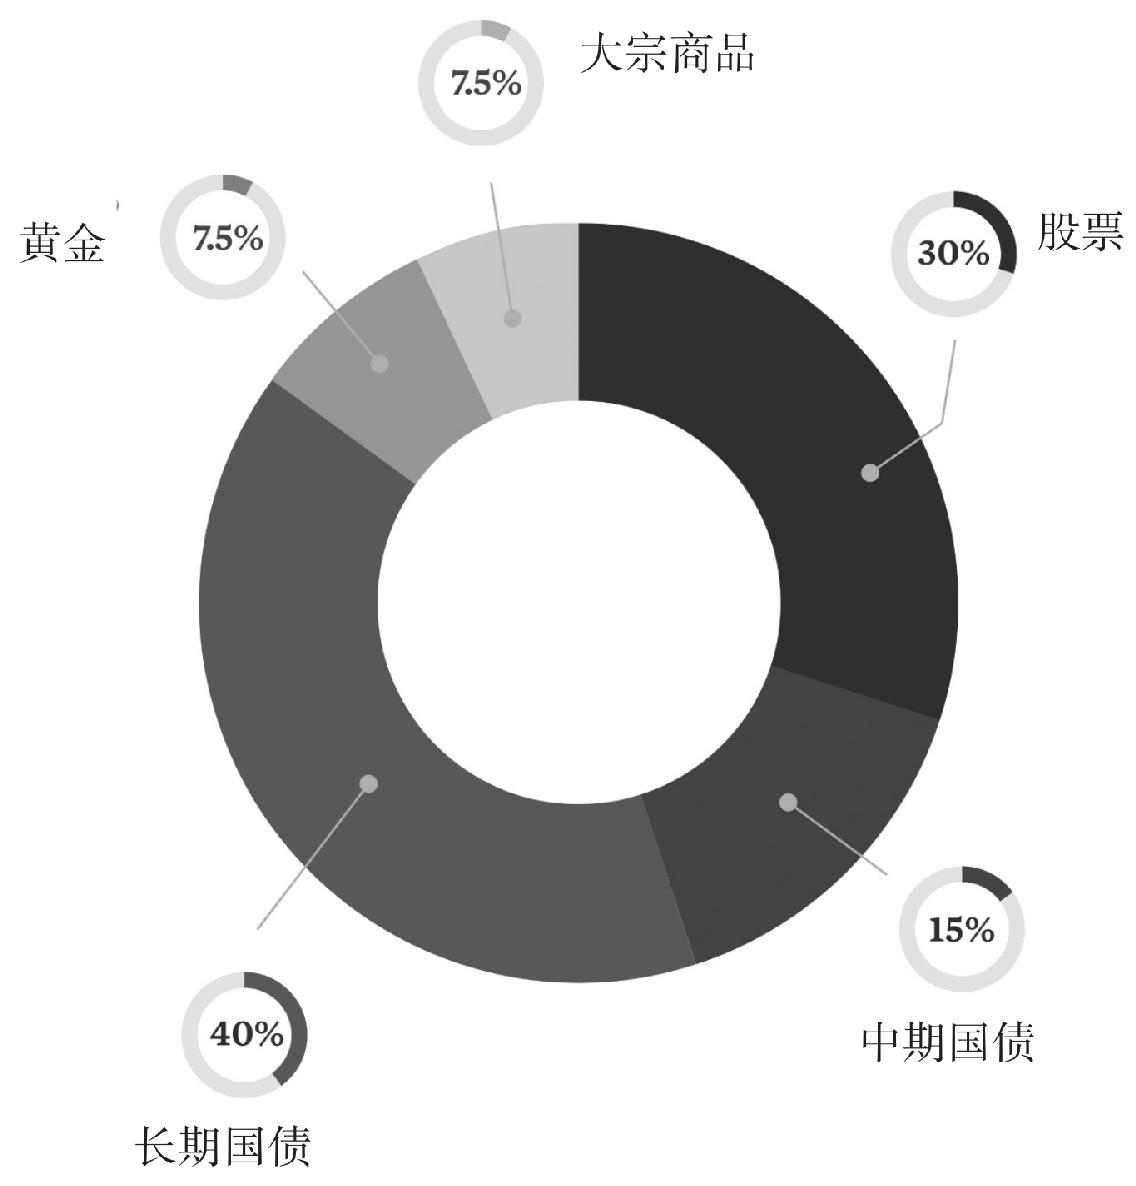
\includegraphics[width=0.6\linewidth,keepaspectratio]{image/26-4.jpg}
\caption{}\label{fig:26-4}
\end{figure}

\subsection{非常感谢}

多少人梦寐以求瑞·达利欧的全天候投资策略对应的明细资产配置方案，现在可是白纸黑字，写得清清楚楚，第一次公开，而且是免费送给各位。瑞·达利欧的投资能力绝对是大师中的大师，而他对待资金少、能力少、经验也少的小投资者却是大度、更大度的，他如此慷慨地提供了一个资产配置方案明细，相当于公布了一个投资秘方，这会改变整个投资界的游戏规则，必将造福数以百万计的中小投资人的人生。你意识到了吧，在那个奇妙的日子里，这个男人提供给我们这样一个资产配置方案，这个行为是多么的慷慨！发自内心地给予，正是瑞·达利欧的价值核心所在。正是出于这个原因，后来我知道瑞·达利欧和他的太太芭芭拉签署了给予誓言，就是比尔·盖茨和巴菲特发起的捐赠承诺——全世界最富有的个人承诺，向慈善事业捐出大部分的个人财富。

\subsection{请注意}

我自己的投资团队对这个全天候投资组合做了历史回测，就是用过去多年的历史数据，相当于重新回到过去，用这个全季节投资组合来做投资，测试其历史业绩表现。我的投资团队把测试结果的数据发给我，我非常震惊。我永远不会忘记那一天。当时我和我太太正在外面共进晚餐，突然收到了我的个人投资理财顾问阿杰伊·古普塔发来的短信：“你能看看邮箱吗？瑞·达利欧分享给你的投资组合，我们做了历史回测，业绩表现数据就在这个邮件里。难以置信！”阿杰伊·古普塔是我多年的投资顾问，办事非常老到，通常晚上不会给我发短信，所以我知道，这肯定不是一般的事情，他才会迫不及待地想马上让我知道。晚餐一结束，我马上抓起我的手机，打开了那封最新邮件……
